\documentclass[11pt,a4paper,fleqn]{article}
\usepackage[margin=1in]{geometry}
\usepackage{graphicx} 
\usepackage{multirow}
\usepackage{hhline}
\usepackage{amsmath}
\begin{document}
\textbf{CS6140 Machine Learning Fall 2014 Homework 2, Wei Luo }\\
\\
\textbf{PROBLEM 1}\\
\\
 \textbf{B)} Training and testing performance across all four learning algorithms is: \\
 
 \hskip-1cm
 \begin{tabular}{|l|l|l|l|l|}
\hline
 &Decision or &Linear Regression &Linear Regression&LogisticRegression\\
 &Regression Tree&(Normal Equations)&(Gradient Descent)&(Gradeint Descent)\\
\hline
Spambase&Train ACC: 0.91&Train ACC: 0.92&Train ACC: 0.91&Train ACC: 0.92\\
&Test ACC: 0.90&Test ACC: 0.88&Test ACC: 0.90&Test ACC: 0.91\\
\hline
Housing&Train MSE: 26.49&Train MSE: 22.08&Train MSE: 22.13&N/A.\\
 &Test MSE: 24.28&Test MSE: 22.63&Test MSE: 22.58&\\
\hline
\end{tabular}\\
\\ \\
 \textbf{C)} \\
 Confusion Matrix for Decision Tree:\\ \\
\begin{tabular}{cc|c|c|}
\multicolumn{2}{c}{}&\multicolumn{2}{c}{Prediction}\\
\multicolumn{2}{c}{}&\multicolumn{1}{c}{1}&\multicolumn{1}{c}{0}\\
\hhline{~~--}
\multirow{2}{*}{Label}
&1&152&29\\
\hhline{~~--}
&0&14&264\\
\hhline{~~--}
\end{tabular}\\ \\
 Confusion Matrix for Linear Regression:\\ \\
\begin{tabular}{cc|c|c|}
\multicolumn{2}{c}{}&\multicolumn{2}{c}{Prediction}\\
\multicolumn{2}{c}{}&\multicolumn{1}{c}{1}&\multicolumn{1}{c}{0}\\
\hhline{~~--}
\multirow{2}{*}{Label}
&1&162&19\\
\hhline{~~--}
&0&22&256\\
\hhline{~~--}
\end{tabular}\\ \\
 Confusion Matrix for Logistic Regression:\\ \\
\begin{tabular}{cc|c|c|}
\multicolumn{2}{c}{}&\multicolumn{2}{c}{Prediction}\\
\multicolumn{2}{c}{}&\multicolumn{1}{c}{1}&\multicolumn{1}{c}{0}\\
\hhline{~~--}
\multirow{2}{*}{Label}
&1&154&27\\
\hhline{~~--}
&0&10&268\\
\hhline{~~--}
\end{tabular}\\ \\
\newpage \noindent
\textbf{D)} \\
ROC curve for Linear Regression:\\
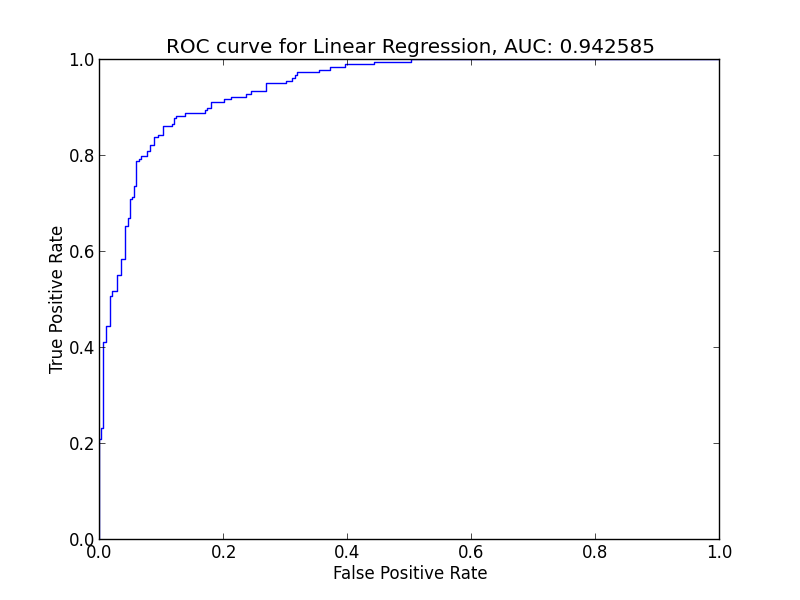
\includegraphics[scale=0.6]{ROC_Linear_Regression.png}\\
ROC curve for Logistic Regression:\\
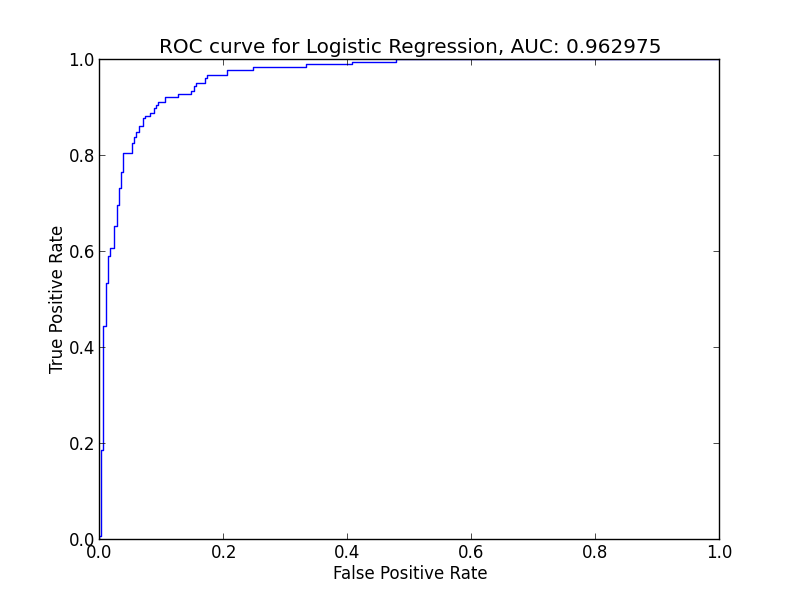
\includegraphics[scale=0.6]{ROC_Logistic_Regression.png}\\
\newpage \noindent
\textbf{PROBLEM 2}\\ \\
Iteration 1, total\_mistake 136\\
Iteration 2, total\_mistake 68\\
Iteration 3, total\_mistake 50\\
Iteration 4, total\_mistake 22\\
Iteration 5, total\_mistake 21\\
Iteration 6, total\_mistake 34\\
Iteration 7, total\_mistake 25\\
Iteration 8, total\_mistake 0\\
Classifier weights:\indent-14.\indent2.52873259\indent5.70717051\indent8.52231457\indent11.32560723\\
Normalized with threshold: \indent0.18062376\indent0.40765504\indent0.60873676\indent0.80897195\\
\\ \\
\textbf{PROBLEM 3}\\ \\
\textbf{b)} 
After training this way, we get a encoder-decoder. With the trained weights, we can encode our data to hidden variables which reduced the size of data. Then the exact data will be kept secret without the weights in our encoder-decoder mechanism. Then, once we need the data, we can decode it with the weights. The weights here are just like keys to encode and decode data.\\
\textbf{c)}
 This encoder-decoder scheme cannot work with one or two hidden variables. Because, the values we get from the sigmoid function is more like binary values. They are distributed near two value. So with $n$ hidden variables, we are more like using $n$ binary values. With that, we can only encode $2^n$ values. So with $N$ input/output values, we need at least $\lceil log_2N \rceil$ hidden variables.\\
\newpage \noindent
\textbf{PROBLEM 4}\\ \\
With our sigmoid function $f(x)$, for a 3-layer neural network, the outputs can be written as
$$g_k(\mathbf{x})=z_k=f(\sum_jw_{kj}f(\sum_iw_{ij}x_i+w_{j0})+w_{k0})$$
The inner $f$ is for hidden variables. If we change it to a linear function, say $lf(x) = ax+b$, then:
\begin{equation}
\begin{aligned}
\nonumber
g_k(\mathbf{x})=z_k&=f(\sum_jw_{kj}lf(\sum_iw_{ij}x_i+w_{j0})+w_{k0})\\
&=f(\sum_jw_{kj}(a_j(\sum_iw_{ij}x_i+w_{j0})+b_j)+w_{k0})\\
&=f(\sum_jw_{kj}(a_j\sum_iw_{ij}x_i+a_jw_{j0}+b_j)+w_{k0})\\
&=f(\sum_jw_{kj}a_j\sum_iw_{ij}x_i+\sum_jw_{kj}(a_jw_{j0}+b_j)+w_{k0})\\
&=f(\sum_i(\sum_jw_{kj}a_jw_{ij})x_i+\sum_jw_{kj}(a_jw_{j0}+b_j)+w_{k0})\\
\end{aligned}
\end{equation}
Let $w'_{ki}=\sum_jw_{kj}a_jw_{ij}$, $w'_{k0}=\sum_jw_{kj}(a_jw_{j0}+b_j)+w_{k0}$, we have
$$g_k(\mathbf{x}) = f(\sum_iw'_{ki}x_i+w'_{k0})$$
Which is equivalent to a two-layer network output.\\
Therefore, a three-layer network with linear hidden units can be reshaped to a two-layer network.\\
With a two-layer network, we cannot solve non-linearly separable problem XOR because: Say, we have weights $w_1\ w_2\ w_3$, basis $b$, and a threshold $t$ for the network. For the XOR problem, we need:\\
\begin{tabular}{cc}
(1) $w_0b+w_10+w_21 \ge t$&(2) $w_0b+w_11+w_20 \ge t$\\
(3) $w_0b+w_10+w_20 < t$&(4) $w_0b+w_11+w_21 < t$\\
\end{tabular}\\
From (1)(2), we have $2w_0+w_1+w_2 \ge 2t$, from (3)(4), we have $2w_0+w_1+w_2 < 2t$ which is a contradiction due to the XOR problem itself is not linearly separable. We can not solve this problem with such network. Similary for other non-linearly separable problems since the function is linear.\\
\newpage \noindent
\textbf{PROBLEM 5} a\\ \\
This lecture notes mainly talks about three major tpoics: \textit{diagnostics for debugging learning algorithms}, \textit{error analyses and ablative analysis} and \textit{how to get started on a machine learning problem}.\\
First, diagnostics for debugging learning algorithms:\\
The motivation problem for this is the anti-spam problem. When using Bayesian logistic regression with gradient descent as the training algorithm the test error is unacceptably high (20\%). 
To imporve this algorithm, there are several common approaches which might work but very time-consuming and may end up with not fixing the problem. 
So a better approach is to run diagnostics to figure out what the problem is.\\
First introduce two common diagnostic variables for the problem: \\
\indent - \textbf{variance} \indent is the variance of features, or the domain of the featueres.\\
\indent - \textbf{bias} \indent\indent\ \  is the importance of some specific features.\\
A high variance indicates overfitting and a high bias indicates there are too few features used to classify spam.\\
The result of high variance is the difference between traing error and test error will be very high. And the result of having a high bais is high training and test errors.\\
Apart from the two variables, we should also care about some other problems like is the algorithm converging? are you using the right objective function? are you using the right learning rate?  Found the problem, we can then use some common ways to fix it.\\
Next, we move on to error analysis:\\
This comes up with an example of face recognition. To analysis the error, you should split the problem into sub-components. Then look into the error for each component and figure out by fixing which component we can make an improvement to the whole problem.\\
For ablative analysis:\\
Instead of evaluating the difference between perfect performance and the current performance, ablative analysis tries to evaluate the difference between some baseline (much poorer) performance and the current performance. By removing components from the system one at a time, ablative analysis can see how much contributions did each component make to your system. Then you can find a better way to improve your system.\\
At last the notes talks about how to get started  on a problem:\\
One approach is careful design. Start a problem with careful design can help your build nicer and more scalable algorithms. The new, elegant learning algorithm may make a difference in machine learning.\\
Another approach is build-and-fix. That is try to get things working as quickly as possible no matter how many problems are there. Then run error analyses and diagnostics to find the problem and fix it. This approach can get your staff to work quickly. Better to use it when the problem is urgent.
\newpage \noindent
\textbf{PROBLEM 5} b\\ \\
The article summarizes twelve key lessons that machine learning researchers and practitioners have learned. Including pitfalls to avoid, important issues to focus on, and answers to common questions.\\
1. Learning includes representation, evaluation and optimization. The first thing we should do in learning is to represent the problem in a way such that the computer can understand it. Then we should develop a function that evaluates the result of our classifier so that we can distinguish  good classifiers from bad ones. Finally, we should find the optimum classifier among the ones we have learned. This process is called optimization.\\
2. Generalization is very important in learning. You can not test the classifier with the data you trained it, your classifier should be able to classy general data not just the data you see. \\
3. Just use data to train your classifier is not enough. Since there are extremely large data around the world, your data can never be big enough to train. Beyond data, you should use some knowledge we already knew about the data, and some assumptions about the data to help you train your classifier.\\
4. Overfitting is a very common problem in machine learning. Bias and variance can help us understand overfitting. And there are some common ways to combat overfitting like cross-validation, add regularization term to the evaluation function, etc. \\
5. Dimensionality is another big problem in machine learning. This refers to the fact that many algorithms that work fine in low dimensions become intractable when the input is high-dimensional. However, most applications examples are running near a lower dimension and there are some algorithms to reduce dimensionality.\\
6. Machine learning problems are always come with theoretical guarantees. You should be careful about those guarantees. The bounds they give is usually too loose, and may result in bad classifier.\\
7. The most important factor in succeeding a machine learning project is the features used. Try to use independent features and avoid complex features. Also, try to find a better way to construct features.\\
8. In order to improve the classifier, it's better to gather more data than to develop a new algorithm. More data can help to build your classifier more scalable.\\
9. You should train your classifier from multiple models not just one. Many techniques exist for model ensembles like bagging, boosting and stacking.\\
10. It is not necessary that when two classifiers have a tie on training error, the simpler one is the better. We prefer simple solutions, but that does not mean simple hypothesis brings more accuracy.\\
11. Representable does not imply learnable. We can always represent a function in some way, but it doesn't mean that the function can be learned. In machine learning, not all functions can be learned.\\
12. Correlation does not imply causation, however, correlation is a sign of potential causal connection, we can use it as a guide for further investigation.\\
\end{document}